\documentclass{beamer}
\usepackage[turkish]{babel}
\usepackage[utf8]{inputenc}
\usepackage[T1]{fontenc}
\usepackage{beamerthemesplit}
\usepackage{graphicx}
\usepackage{graphics}

\title{Linux Nedir?}
\author{Ahmet Emre Aladağ}
\date{13-16 Ekim 2008}
\institute{emre.aladag at isik.edu.tr \newline \newline Işık Üniversitesi Bilgisayar Kulübü\\http://bilgisayar.isikun.edu.tr \newline \newline IŞIX\\http://isix.isikun.edu.tr}
% \place{Işık Üniversitesi}
% \date{\today

\begin{document}

\frame{\titlepage}
\part{3N1K}
\begin{frame}

\begin{center}
\large 3N 1K
\end{center}

\end{frame}
\section[Genel Bakış]{}
\frame{\footnotesize\tableofcontents}



\section{Nasıl?}
	\subsection{Özgür Yazılım (Free Software)}
		\begin{frame}
			\frametitle{Özgür Yazılım ve Tarihçesi}
			\begin{columns}
			\begin{column}[l]{5cm}
				\begin{itemize}
				\item UNIX pahalı, özgür değil
				\item Özgür bir işletim sistemi yazacağız!
				\item Yazılım topluma ait olmalı...
				\end{itemize}
			\end{column}
			\begin{column}[r]{5cm}
			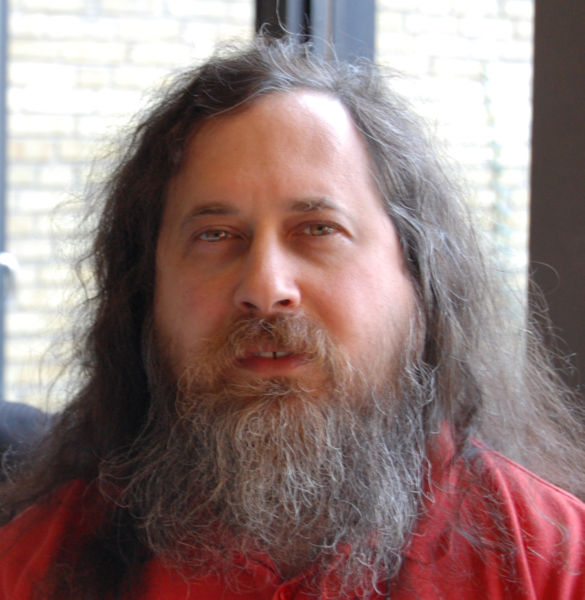
\includegraphics{richard}
			\end{column}
			\end{columns}
			
		\end{frame}
		
	\subsection{GNU}
		\begin{frame}
		 	\frametitle{GNU Projesi ve GPL}
			\begin{columns}
			\begin{column}[l]{5cm}
				\begin{itemize}[<+->]
					\item UNIX Modeli
					\item GNU's NOT UNIX
					\item İşletim Sisteminin Çekirdek (Kernel) Dışındaki Parçaları
					\item GPL(Genel Kamu Lisansı) 1991
					\item Linux Çekirdeği ve Bütünleşme
				\end{itemize}
			\end{column}
			\begin{column}[r]{5cm}		
				
\includegraphics{gnukucuk.jpg}
			\end{column}
			\end{columns}


		\end{frame}
	\subsection{GPL}
		\begin{frame}
		 	\frametitle{GPL (General Public Licence)}
			\begin{itemize}
			 \item Programı her türlü ihtiyaç için çalıştırma
			 \item İhtiyaçlarına göre değiştirebilme
			 \item Arkadaşlarınızla paylaşabilme
			 \item Değiştirdiğiniz halini tekrar paylaşabilme ve hatta satabilme
			\end{itemize}

		\end{frame}


	\subsection{Açık Kaynak (Open Source)}
		\begin{frame}
		 	\frametitle{Açık Kaynak Kodlu Yazılım}
			\begin{itemize}
			 \item Özgür Yazılımdan Farklı
			 \item Kodlar Açık
			 \item Dağıtma izni olmayabilir
			 \item Kaynağın açık olması güvenilirliği arttırır
			 \item Microsoft Açık Kaynak iş modelinden şikayetçi ama mecburen açık kaynağa yöneliyor.
			\end{itemize}
		\end{frame}
	\subsection{Yönetici Aranıyor}
		\begin{frame}
		 	\frametitle{GNU hazır, peki ya Linux?}
				\begin{itemize}[<+->]
				\item Programlar hazır
				\item Yönetecek çekirdek yok!
				\item Linus devreye giriyor
				\end{itemize}
		\end{frame}
		\begin{frame}
		 	\frametitle{Linus Torvalds}
				\begin{center}
					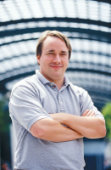
\includegraphics{linus.jpg}
				\end{center}
		\end{frame}
		



\section{Ne?}
	\subsection{İşletim Sistemi (Operating System)}
%		\includegraphics{trafikcanavari.jpg}
		\begin{frame}
			\frametitle{İşletim Sistemi Nedir?}
			\begin{itemize}[<+->]
			 \item Patron
			 \item Trafik Polisi 
			 \item Çevirmen
			 \item Muhatabınız 
			 %Sizin bilgisayar sandığınız şey. Aslında yok öyle iki tıkla program açmak
			\end{itemize}

		\end{frame}

	\subsection{Çekirdek}
		\begin{frame}
		 	\frametitle{Çekirdek Nedir? Yenir mi?}
			\begin{itemize}[<+->]
			 \item Aslında Linux=Çekirdek
			 \item Sürücüleri (Driver)  içerir
			 \item Modüler bir yapıdadır
			 \item Donanım Yönetimi (Bellek, İşlemci, Görüntü, Ağ, ...)
			 \item Donanım - Yazılım İletişimi			 
			 \item Linux 2.6
			 \item Her yerde kullanılıyor: PC'ler, Google Android, Cep Telefonları, PDA'ler, Casio Hesap Makineleri, Uzay Mekikleri, Robotlar
			 

			\end{itemize}
			
		\end{frame}

	\subsection{GNU/Linux}
		\begin{frame}
		\begin{center}
 		 
\includegraphics{linux.png}
		\end{center}
		\end{frame}

		\begin{frame}
			\frametitle{Linux Nasıl Ortaya Çıktı?}
			%\begin{columns}
			 %\begin{column}[l]{7cm}
				\begin{itemize}
					\item Linus Torvalds ve Yetersiz Minix
					\item Yeni bir çekirdek
					\item Linus + UNIX = Linux
					\item Laynıks, Lünüks değil; Linuks, Lihnuks
				\end{itemize}  
			 %\end{column}
			%\begin{column}[r]{5cm}
			 %\includegraphics*[0in,0in][10in,10in]{linus.jpg}
			%\end{column}

			%\end{columns}


		\end{frame}
	
	\subsection{Dağıtım (Distribution)}
		\begin{frame}
		 	\frametitle{Dağıtım Nedir? Neleri içerir?}
			Dağıtım = Çekirdek ve Uygulamalar paketi.\\ Uygulamalar ihtiyaca göre seçilir. Dağıtımlar şu araçları içerir:\\
			\begin{itemize}[<+->]
			 \item Kurulum Aracı (Installer)
			 \item Çekirdek (Kernel)
			 \item Uygulamalar (Applications)
			 \item Yapılandırma Araçları (Configuration Tools)
			 \item Paket Yöneticisi (Package Manager)
			\end{itemize}

		\end{frame}
		
		\begin{frame}
		 	\frametitle{Dağıtımlar}
			\begin{itemize}
			 \item Pardus
			 \item Ubuntu ve Türevleri
			 \item SuSE
			 \item RedHat
			 \item Arch
			 \item Debian
			 \item Gentoo
			 \item Fedora
			 \item Slackware
			 \item PCLinuxOS
			 \item Turkix
			 \item Gelecek Linux
			\end{itemize}
		\end{frame}


	\subsection{Masaüstü Ortamı (Desktop Environment)}
		\begin{frame}
		 	\frametitle{Masaüstü Ortamları}
				\begin{itemize}
				 \item KDE
				 \item Gnome
				 \item Xfce
				 \item Enlightenment
				\end{itemize}

		\end{frame}


\section{Neden?}
	\subsection{Neden Linux?}
		\begin{frame}
		 	\frametitle{Sebep?}
			\begin{itemize}[<+->]
			 \item Virüslerden korunmak için (format yok!)
			 \item Sistem istikrarı ve başarım için (defrag yok! donma yok!)
			 \item Tasarruf için (lisans ücreti yok!)
			 \item Sistemle beraber her şeyin(program ve sürücüler!) hazır gelmesi için (ek kurulum yok!)
			 \item Tüm yazılımlarınızı birkaç tıkla güncelleyebilmeniz için
			 \item Korsan yazılım kullanmamak için
			 \item Program aramaktan bıkmamak için
			 \item Düşük donanımla yüksek kalite masaüstleri için (para vermek yok!)
			 \item Özgürlük için (beklemek yok!)
			 \item Mutlu olmak için
			 \item Yan etkisi: araştırmacı ruhun ortaya çıkması
			\end{itemize}

		\end{frame}
		\begin{frame}
		 \begin{center}
			 
\includegraphics{bgl.png}
		\end{center}
		
		\end{frame}

	%\subsection{Neden Mac?}
	\subsection{Neden Windows?}
		\begin{frame}
		 	\frametitle{Niye ki?}
			\begin{itemize}[<+->]
			 \item İflah olmaz bir oyun hastasısınız (Cedega)
			 \item Bazı programların Linux karşılığı yok (Wine)
			 \item Donanımınız Linuxla anlaşamadı (Hata raporu)
			 \item Yedekte dursun diye (Hepimiz insanız)
			 \item Microsoft'a hayransınız (E, olabilir...)
			 \item Para harcamaktan hoşlanıyorsunuz (Yok artık!)
			\end{itemize}

		\end{frame}
	
	\subsection {Linux'un Eksileri}
		\begin{frame}
			\frametitle{Nesi eksik ki?}
			\begin{itemize}[<+->]
			 \item Donanım Uyuşmazlığı (Üstesinden gelinebilir)
			 \item Paket standardının olmaması (Virüslere engel)
			 \item Web-cam desteği (Skype)
			 \item Bazı programların Linux sürümünün olmaması (Kullanıcı az)
			\end{itemize}

		\end{frame}



\section{Kim?}
	\subsection{Türkiye'de}
		\begin{frame}
		 
			\frametitle{Türkiye'de Kim Kullanıyor?}
			\begin{columns}
			\begin{column}[l]{5cm}
				\begin{itemize}
					\item MİT
					\item Türk Silahlı Kuvvetleri
					\item Başbakanlık
					\item TCMB
					\item TÜBİTAK
					\item Tepe İnşaat
					\item Show TV
				\end{itemize}
			\end{column}
			\begin{column}[r]{5cm}
				\begin{itemize}

					\item Finansbank
					\item HSBC
					\item Citibank
					\item Ziraat Bankası
					\item ODTÜ
					\item İTÜ
					\item ÇOMÜ
					\item Bilgi Üniversitesi
				\end{itemize}
			\end{column}
			\end{columns}

		\end{frame}

	\subsection{Dünya'da}
		\begin{frame}
		 	\frametitle{Linux'u Dünya'da Kim Kullanıyor?}
			\begin{columns}
			\begin{column}[l]{5cm}
				\begin{itemize}
					\item NASA
					\item Google
					\item IBM
					\item Yahoo
					\item HP
					\item Oracle
					\item Novell
					\item Troll Tech
				\end{itemize}
			\end{column}
			\begin{column}[r]{5cm}
				\begin{itemize}
					\item Nokia
					\item Sony Ericsson
					\item Siemens
					\item Samsung
					\item Boeing
					\item General Motors
					\item Hyundai	
				\end{itemize}
			\end{column}
			\end{columns}

		\end{frame}
\part{SON}
\section {Hadi Bakalım}
	
	\subsection{Nasıl Deneyeceğim?}
	\begin{frame}
		\frametitle{İşte Böyle}
			\begin{itemize}[<+->]
			\item Çalışan(Live) CD'ler
			\item Vmware / Virtual Box (Virtualization)
			\item Gerçek Kurulum
			\begin{itemize}
 				\item Tüm diske
				\item Windows'un yanına ayrı bir bölüme (partition)
			\end{itemize}

			%Pardus'un sitesinden
			\end{itemize}
	\end{frame}

	\subsection {Yardım?}
	\begin{frame}
		\frametitle{Nasıl yardım alacağım?}
		\begin{itemize}[<+->]
		 \item \color{brown}Google
		 \item \color{brown}ARANAN site:liste.pardus.org.tr
		 \item Pardus WIKI - http://tr.pardus-wiki.org
 		 \item Özgürlük İçin - http://www.ozgurlukicin.com -> İlk Adımlar
		 \item Pardus Kullanıcıları Listesi - http://liste.pardus.org.tr/pardus-kullanicilari
		 \item IRC Sohbet Kanalı - irc.freenode.org \#pardus
		 \item \color{black}Linux Kullanıcıları Listesi - http://liste.linux.org.tr
		 \item Diğer Forumlar
		 \item Kurumsal Destek: SuSE(Novell), Gelecek Linux(Gelecek A.Ş.)
		 \item \color{brown}IŞIX - http://isix.isikun.edu.tr 
			 
		\end{itemize}

	\end{frame}
	
	\subsection{Siz sormadan...}
	\begin{frame}
	 	\frametitle{Siz sormadan cevaplayayım}
		\begin{itemize}[<+->]
			\item Linux ile her şeyi yapabilir miyim?
			\item Linux gerçekten hiç çökmüyor mu?
			\item Linux bu kadar iyi ise neden herkes Windows kullanıyor?
			\item Linux, Microsoft'a bir tepki mi?
			\item Microsoft'ta teknik desteği kurumdan alabiliyorum, Linux'ta üst merci olarak nereye başvuracağım?
			\item Neden tek bir Linux dağıtımı yok? (Değiştirme özgürlüğü)
			\item Linux ne zaman paralı olacak?
			\item Deli mi bu özgür yazılımcılar? Aç kalmıyorlar mı? (follars.com)
		\end{itemize}

	\end{frame}
	
% --------------------PARDUS----------------------------------
	\subsection{Pardus}
	\begin{frame}
	 
\includegraphics{pardus.jpg}
	\end{frame}

	\begin{frame}
	 	\frametitle{Pardus: Uludağ}
		\begin{itemize}[<+->]
		 \item TÜBİTAK tarafından
		 \item Ulusal dağıtım
		 \item Pardus 2008.1: http://www.pardus.org.tr
		 \item 30 dakikada tam Türkçe ve diğer dil destekleri ile gerekli tüm programlar...
		 \item Türkçe dil denetimi: Zemberek
		 \item Python ile kendi araçlarını yazıyorlar: Yalı, Kahya, Sahip, Pisi, Tasma, Çomar, Müdür, Muavin, Ağ/Paket/Kullanıcı/Açılış Yöneticisi, Güvenlik Duvarı,...
		 \item Staj programı
		 \item Pardus Genişliyor: ASAL, Devlet daireleri, okullar, ...		 
		\end{itemize}

	\end{frame}
	\begin{frame}
	 \frametitle{Nasıl katkıda bulunabilirsiniz?}
		\begin{itemize}[<+->]
		 \item Öncelikle Kullanarak
		 \item Pardus'u tanıtma ve kurulumu/kullanımında yardımcı olma
		 \item Okulda kullanımı için destekleme (Bölüm başkanları/BIM)
		 \item Çeviri çalışmaları (KDE, Pardus, Gnome, ...)
		 \item Hata/İyileştirme raporu girme (http://hata.pardus.org.tr)
		 \item Yeni özellik önerme (http://www.ozgurlukicin.com -> Beyin)
		 \item Hata düzeltme
		 \item Paket Yapma
		 \item Yazılım geliştirme
		\end{itemize}

	\end{frame}

	\begin{frame}
	\frametitle{Başkalarının dilinden}
	... Ben de Pardus'a geçtiğimde önceleri sizin gibi
	düşünmüştüm. Ama kısa zamanda alıştım ve şimdi bunca yıl neden Windows'la
	zaman kaybetmişim diye düşünüyorum. Çünkü çok kısa zamanda alışılıyor. Ve
	görülüyor ki Pardus aslında çok daha kolay ve pratikmiş. Hele virüs tehdidi
	olmayışı olağanüstü bir rahatlık veriyor.
	
	Zaten Windows'un yeni versiyonlarına da alışmak için belli bir süre gerekiyor.
	Aynı süreyi Pardus için ayırırsak, her şey halloluyor.
	\newline
	\newline
	Emre Kocaoglu
	\newline
	21. Dönem İstanbul Milletvekili
	\end{frame}
	
	\begin{frame}
	 \frametitle{Kurulumu}
		\begin{itemize}
		 \item http://www.pardus.org.tr -> İNDİR -> Kurulum Kılavuzu
		 \item http://www.ozgurlukicin.com -> İlk Adımlar
		 \item http://isix.isikun.edu.tr
		 \item Bizzat bizden yardım isteyerek
		\end{itemize}

	\end{frame}


% -------------------------------------------------------------
	\subsection{Sana nasıl ulaşabiliriz?}
	\begin{frame}
	 	\frametitle{Kimsin sennn?}
		\begin{quote}
 			Ahmet Emre Aladağ \\ emre.aladag at isik.edu.tr \\ http://www.emrealadag.com\\
		\end{quote}
	\end{frame}
	\begin{frame}
	 \frametitle{Kim Korkar Bilgisayar Kulübünden?}
			16 Ekim Perşembe 17.00 - DMF-114
			\begin{itemize}
				\item Tanışma
				\item Üyelik
				\item Etkinlik istekleri
				\item Özgür Yazılım Takımı
			\end{itemize}
	\end{frame}
	\begin{frame}
		\frametitle{Şimdi?}
	 	Kurulum Görüntüleri\\
		Perşembe 11-13\\
		Sunum\\
		Yurt.NET
	\end{frame}

	\subsection{Sorularınız?}
	\begin{frame}
	 	\frametitle{Sorularınız...}
		\begin{center}
		 ?
		\end{center}
		
	\end{frame}


\end{document}
    